\chptr{Meccanica degli Urti}
\marginpar{\minitoc}

Fino ad ora abbiamo trattato il moto di corpi ``solitari'', ovvero non
perturbati da altri corpi, ma al massimo influenzati da qualche agente
esterno (le forze). Trattiamo ora gli urti, fenomeni dei quali abbiamo
un'idea intuitiva secondo la quale lo ``scontro'' determina un qualche
cambiamento nella velocità e nella traiettoria degli oggetti coinvolti.
Per trattare gli urti è necessario introdurre due nuove grandezze:
Quantità di moto e impulso.


\section{Quantità di moto}
Abbiamo sempre espresso la seconda legge come
\[ \vecsymb{F} = m\vecsymb{a} = m\frac{d\vecsymb{v}}{dt} \]
ma questa proposizione afferma che l'effetto dell'agente esterno (la forza
$\vecsymb{F}$) si traduce interamente in una variazione dello stato di
moto del corpo (accelerazione $\vecsymb{a}$). Si suppone quindi che la
massa sia sempre costante, anche se ciò non è sempre vero. Ad esempio,
un razzo pieno di carburante non avrà la stessa massa che aveva in partenza
una volta arrivato in orbita, quindi la forza esercitata dalla propulsione
dei motori si è tradotta non solo in una variazione dello stato di moto,
ma anche in una variaizione della massa. Non tratteremo sistemi complessi
come il razzo, ma ciò fa intuire che la seconda legge della dinamica può
essere generalizzata nella forma seguente
\begin{align}
    \vecsymb{F} = \frac{d}{dt}(m\vecsymb{v}) = \frac{d\vecsymb{p}}{dt}\label{qtamotosecondalegge}
\end{align}
Dove la quantità $\vecsymb{p}$ prende il nome di \textit{quantià di moto},
definita come
\begin{align}
    \vecsymb{p} \eqdef m\vecsymb{v}
\end{align}
Come dice il termine, la quantità di moto descrive il moto dei corpi
sulla base della velocità di una massa più la massa stessa, a differenza
di quanto accade nello studio cinematico del moto, dove solo le variazioni
dello stato di moto contano, slegate da cause (forze) e materia (massa).
La quantità di moto è inoltre una grandezza vettoriale, perché contiene
in sé la velocità, a sua volta grandezza vettoriale.

%L'effetto della quantità di moto si percepisce in molte situazioni quotidiane.
%Nel bowling, possiamo incassare uno strike perché il moto della palla viene
%trasmesso ai birilli, che a loro volta vengono messi in moto e dunque cadono.
%Se immaginiamo di essere su uno skateboard, in grado di muoversi su un piano
%senza attrito, e chiediamo ad un amico di passarci una palla, è sicuro che
%una volta afferrata la palla lo skateboard sul quale ci troviamo comincerà
%a muoversi. Esso sarà inoltre tan


\section{Impulso}
In molte situazioni comuni le forze agiscono per un tempo brevissimo, come
negli urti. In questi casi è utile introdurre la grandezza dell'impulso.
Supponiamo, ad esempio, che in una partita di baseball il lanciatore faccia
partire la palla a una velocità di 150 km/h. Il battitore ruota il braccio
e colpisce con la mazza la palla, che ritorna verso il lanciatore a 185 km/h.
Nel breve intervallo di tempo durante il quale la palla e la mazza sono in
contatto, dell'ordine del millesimo di secondo, la forza fra esse cresce
rapidamente fino ad un valore massimo molto grande, quindi si annulla quando
la palla si stacca dalla mazza.

Descrivere l'andamento nel tempo della forza che la mazza esercita sulla palla è
difficile. Ciò che possiamo conoscere più facilmente con una strumentazione
adeguata è la \textit{variazione della quantità di moto} (massa e velocità) della
palla a causa del colpo e il tempo $\Delta t$ di contatto tra mazza e palla. Da questi
dati possiamo allora accontentarci di ottenere, usando l'equazione \ref{qtamotosecondalegge} una \textit{forza media}, ovvero
una forza che si è mantenuta costante per tutto l'intervallo di tempo del contatto
mazza-palla.

\[ \left\langle \vecsymb{F}\right\rangle  = \frac{\Delta\vecsymb{p}}{\Delta t} \]

\noindent Riformulando questa equazione per variazioni infinitesime, possiamo
ottenere la variazione di quantità di moto in funzione di $\vecsymb{F}$ e $dt$:

\[ d\vecsymb{p} = \vecsymb{F}dt \]

\noindent Il prodotto $\vecsymb{F}dt$ viene definito \textit{impulso} e non è
altro che una definizione matematica alternativa della variazione della quantità
di moto, utilizzata però più spesso in contesti in cui agiscono forze \textit{impulsive},
cioè forze variabili che agiscono per tempi molto brevi rispetto a quelli
comunemente misurabili nel sistema esaminato.

\begin{align}
    \vecsymb{I} \stackrel{\text{def}}{=} \vecsymb{F}dt
\end{align}

\noindent L'impulso è particolarmente utile per spiegare il motivo per cui
è più confortevole atterrare su 10 metri di neve dopo una caduta di 100 metri
piuttosto che su una lastra di pietra. Per frenare la nostra caduta, la neve
ci permette di sprofondare al suo interno, quindi essa varia la nostra quantità
di moto in maniera graduale e su un intervallo di tempo prolungato. Al contrario,
la lastra di pietra non si deforma in maniera apprezzabile e l'impatto determina
un impulso molto forte rispetto alla neve, tanto da essere letale.


\section{Il fenomeno dell'urto}

\begin{tcolorbox}[colback = yellow!30, colframe = yellow!30!black, title = {Urto}]
    Un urto è un'interazione tra corpi, nella quale si osservano forze
    denominate \textit{impulsive}, che cioè agiscono per tempi e su distanze
    molto più brevi di quelli \textit{tipici} osservabili all'infuori
    dell'urto.
\end{tcolorbox}
\vspace{5pt}

Cosa si intende per distanze e tempi tipici? Per i lettori che ancora si
ricordano, immaginiamo una puntata di Holly \& Benji: Quando i calciatori
si apprestano a sferrare un calcio, il disegnatore sceglie sempre
di rappresentare l'istante del colpo deformando il pallone. Anche se questa
raffigurazione è evidentemente esagerata, essa ha un fondo di verità e offre una spiegazione
intuitiva di cosa si intende per \textit{distanze tipiche dell'urto}: in un
urto, gli oggetti coinvolti si \textit{deformano}. Queste deformazioni avvengono
su distanze ben minori di quelle, per esempio, della traiettoria del calcio o
della lunghezza del campo. In urti reali, inoltre,
come il calcio alla palla di Holly \& Benji, queste deformazioni sono inevitabili,
nonostante i corpi che collidono sembrino apparentemente i più rigidi su
questo pianeta\footnote{Il suono è prova del fatto che sono avvenute vibrazioni
nei corpi, che dunque si sono deformati.}. Bisogna poi specificare che le
deformazioni sono molto difficili da osservare perché, oltre ad avvenire su
distanze ridotte rispetto a quelle tipiche, anche i tempi nelle quali accadono
sono molto brevi. Il contatto tra piede e pallone è molto ridotto rispetto a
quello che invece è richiesto al calciatore per correre dall'angolo al centro
del campo. Riassumendo questo esempio calcistico, quando osserviamo una
partita siamo di fronte a grandezze \textit{tipiche} (dimensioni del campo da
calcio, velocità dei calciatori e della palla, ecc.); negli urti, invece,
possiamo trascurare le deformazioni e le distanze, perché troppo piccole
rispetto a quelle tipiche, e i tempi, perché gli urti appaiono come eventi
istantanei ai nostri occhi.

L'intenzione della meccanica di questo capitolo, dunque, non è quella di
descrivere ciò che accade \textit{durante} l'urto, ma prevedere, date le
informazioni \textit{precedenti} all'urto, lo stato del sistema
\textit{successivamente} all'urto. Idealmente, l'urto avviene istantaneamente
e i corpi coinvolti sono sempre punti materiali, che dunque non conoscono
deformazioni.

\subsection*{Urti e quantità di moto}
Vogliamo prevedere lo stato del sistema dopo l'urto, in termini di
velocità (vettori) dei corpi coinvolti. Sorprendentemente, gli unici
strumenti che servono per trattare in modo semplice questo problema
sono i tre principi della dinamica, più la definizione di quantità
di moto e l'assunzione del \textit{sistema isolato}, ovvero non
disturbato da forze esterne.

Un classico esempio che unisce nozioni su urti e quantità di moto è il
tavolo da biliardo. Supponiamo di avere due palle, 1 e 2, sul tavolo in moto
rettilineo
uniforme e in rotta di collisione tra loro; ovvero, sappiamo con certezza
che la loro traiettoria si intersecherà e che tale punto verrà raggiunto
da entrambi i corpi nel medesimo istante di tempo. L'esprerienza ci permette
di concludere che, passata la \textit{zona d'urto}, le palle non procederanno
sulle stesse rette dei moti precedenti, ma devieranno.
Dobbiamo fare alcune assunzioni fondamentali. Innanzitutto, supporremo che
nessun altro agente agirà sul sistema appena descritto (aiuterebbe immaginare
due palle che vagano nello spazio profondo, o in altre parole: Nulla deve
disturbare il sistema).
Immaginiamo l'intervallo temporale nel quale le due palle saranno a contatto
tra loro, collidendo: entrambe eserciteranno una forza sull'altra e aiutati
dalla terza legge della dinamica sappiamo che

\[ \vecsymb{F}_{1 \to 2} = -\vecsymb{F}_{2 \to 1} \]

\noindent cioè l'applicazione di una forza su una palla determina una forza identica
in modulo e direzione, ma verso opposto e applicata sull'altra palla.
Sviluppiamo l'equazione sfruttando la definizione di quantità di moto,
ricordando che una forza $x \to y$ determina una variazione dello stato di
moto di $y$.
\[ \frac{d\vecsymb{p}_2}{dt} = -\frac{d\vecsymb{p}_1}{dt} \]
Ricorrendo agli usuali abusi di notazione matematica, ma ragionevoli da
un punto di vista fisico, semplifichiamo l'intervallo di tempo infinitesimale
del differenziale:
\begin{align*}
    &d\vecsymb{p}_2 = -d\vecsymb{p}_1\\
    &d[\vecsymb{p}_1 + \vecsymb{p}_2] = 0\\
    &d\vecsymb{p}_\text{tot} = 0
\end{align*}
Abbiamo mostrato, in anticipo, che per un sistema di due corpi come le palle
da biliardo, assumendo che non agiscano forze esterne, la quantità di moto
totale del sistema si conserva. Come l'energia meccanica, possiamo dunque
concludere che un urto ideale non modifichi la quantità di moto del sistema.
Questa conclusione è ancora incompleta e inesatta perché, come scopriremo
in una prossima sezione, la quantità di moto si conserva \textit{sempre} in
un sistema isolato e non dipende dalla natura dell'urto.

\section{Conservazione}
Come l'energia, nella storia della fisica si è sempre pensasto al moto
come una quantità che potesse essere trasferita da un corpo ad un altro,
fatto ragionevole ben giustificato dall'esperienza: basti pensare al
gioco del biliardo.
Come già dedusse Cartesio, la ``macchina dell'universo'', assimilata ad
un orologio, non può continuare a funzionare senza che una qualche quantità
si conservi. Egli stesso fu tra i primi a proporre il prodotto massa-velocità
come misura di tale quantità: due carri identici che viaggiano a velocità differenti
hanno chiaramente quantità di moto diverse, ma una palla di cannone
racchiude in sé maggior moto rispetto ad un sasso lanciato alla stessa
velocità. Queste quantità sono presenti negli oggetti secondo distribuzioni
differenti e variabili nel tempo, ma nel complesso esse non possono che
sommarsi (vettorialmente!) sempre nella medesima quantità; se l'universo è un
sistema chiuso, e lo si può supporre per definizione, allora la quantità di moto
non può sparire o comparire, ma può trasferirsi tra gli oggetti al suo
interno, trasformarsi.

\subsection{Forze interne ed esterne}
Approfondiamo il concetto di \textit{sistema di punti materiali} e studiamone
uno contentente un certo numero di punti materiali $N$. Immaginiamo che
tra questi punti agiscano forze di varia natura: repulsive elettriche,
attrattive gravitazionali ecc.; inoltre, supponiamo che vengano applicate
altre forze dall'esterno di questo sistema di punti materiali\footnote{Una
immagine esplicativa è il polmone, dove le molecole dell'aria formano i
punti materiali e i muscoli del torace sono gli agenti esterni.}.
Possiamo suddividere le forze in gioco in due insiemi:
\begin{enumerate}
    \item \textbf{Forze interne}: le forze che i punti esercitano gli uni
    sugli altri. Forze che descrivono l'interazione tra i punti.
    \item \textbf{Forze esterne}: le forze che l'ambiente esterno esercita
    sul sistema, l'insieme di punti.
\end{enumerate}
Ogni punto $i$-esimo sarà sottoposto ad una certa forza totale, o risultante, derivante
dalla somma/sovrapposizione di tutte le forze precedentemente descritte
\begin{align*}
    \vecsymb{R}_i = m_i\vecsymb{a}_i\\
    \vecsymb{R}^{(E)}_i + \vecsymb{R}^{(I)}_i = m_i\vecsymb{a}_i
\end{align*}
Definiamo le risultanti delle forze esterne, ed interne agenti sul punto
$i$-esimo:
\begin{align*}
    \vecsymb{R}^{(E)}_i &\eqdef \sum_{k} \vecsymb{F}^{(E)}_{k \to i}\\
    \vecsymb{R}^{(I)}_i &\eqdef \sum_{j} \vecsymb{F}^{(I)}_{j \to i} \qquad j \not = i
\end{align*}
Supponiamo che un punto non eserciti alcuna forza su se stesso (per questo
poniamo $i \not = j$).
La risultante di tutte le forze in gioco sarà
\[ \vecsymb{R} = \sum_{i} \vecsymb{R}_i \]
In tale somma, concentriamoci sulla risultante delle forze interne:
\[ \vecsymb{R}^{(I)} = \sum_{i} \vecsymb{R}^{(I)}_i = \sum_{i} \sum_{j} \vecsymb{F}^{(I)}_{j \to i} \]
In questa somma, supponiamo che non vi siano forze agenti su un corpo
ed esercitate dal corpo stesso, dunque poniamo $\vecsymb{F}^{(I)}_{j \to i} = \overrightarrow{0} \quad \forall j = i$.
Sappiamo che vale la terza legge della dinamica, dunque
$\vecsymb{F}^{(I)}_{j \to i} = -\vecsymb{F}^{(I)}_{i \to j}$. Ma allora
\begin{align}
    \vecsymb{R}^{(I)} = \sum_{i} \sum_{j} \vecsymb{F}^{(I)}_{j \to i} = \overrightarrow{0}\label{interne}
\end{align}
Abbiamo appena dimostrato, grazie all'ipotesi della terza legge,
che, in un sistema di punti materiali, la risultante delle forze interne
è nulla.

\subsection{Centro di massa}
Dall'Equazione \ref{interne} possiamo dedurre che la risultante delle
forze, interne ed esterne, coinvolte in un sistema di punti materiali
è determinata solamente dalle forze esterne.
\[ \vecsymb{R} = \vecsymb{R}^{(E)} = \sum_{i} \vecsymb{R}^{(E)}_i = \sum_i m_i\vecsymb{a}_i \]
Dalla precedente equazione, si può ricavare un'interessante definizione:
\[ \sum_i m_i\vecsymb{a}_i = \sum_i m_i \frac{d^2\vecsymb{x}_i}{dt^2} = \left(\sum_i m_i\right) \frac{d^2}{dt^2}\left[ \frac{\sum_i m_i\vecsymb{x}_i}{\sum_i m_i} \right] \]
Abbiamo ottenuto un termine molto interessante, un artificio matematico
che ha interpretazioni e applicazioni piuttosto importanti: \textit{il
centro di massa}.
\begin{align}
    \vecsymb{x}_\text{CM} \eqdef \frac{\sum_i m_i\vecsymb{x}_i}{\sum_i m_i}
\end{align}
Dalla definizione è banane\footnote{Hai letto bene.} ricavare la velocità e l'accelerazione del
centro di massa. Riprendendo le equazioni precedenti e ponendo $M = \sum_i m_i$,
possiamo concludere che
\[ \vecsymb{R}^{(E)} = M\frac{d^2\vecsymb{x}_\text{CM}}{dt^2} = M\vecsymb{a}_\text{CM} \]

\subsection{La legge di conservazione della quantità di moto}
In un sistema isolato, non si rilevano forze esterne. Allora
\[ \vecsymb{R}^{(E)} = \overrightarrow{0} \quad \therefore \quad M\vecsymb{a}_\text{CM} = 0 \quad \therefore \quad \vecsymb{a}_\text{CM} = 0 \]
ovvero, la velocità del centro di massa è costante, quindi la
quantità di moto del centro di massa è costante e si conserva in
un sistema isolato. Vale dunque la seguente:

\begin{align*}
    \vecsymb{v}_{\text{CM}, i} &= \vecsymb{v}_{\text{CM}, f}\\
    \frac{\sum_j m_j\vecsymb{v}_{j,i}}{M} &= \frac{\sum_j m_j\vecsymb{v}_{j,f}}{M}\\
    \vecsymb{p}_{\text{tot}, i} &= \vecsymb{p}_{\text{tot}, f}
\end{align*}

\noindent Da cui

\begin{align}
    \frac{d}{dt}\vecsymb{p}_\text{tot} = 0
\end{align}
Tale risultato ha conseguenze di portata non trascurabile. Si consideri
infatti il problema esposto nella prossima sottosezione.

\subsubsection*{Punto di collisione}
Due magneti di massa $m$ e $5m$ sono mantenuti ad una distanza fissa tra
di loro. Una volta rimossi i vincoli, i due magneti si attraggono fino a
schiantarsi. Sapendo che il primo magnete si trovava in posizione $x_1 = 0$
mentre il secondo in $x_2 = 8\text{ cm}$, si intende individuare la posizione
della collisione.

Alla luce della legge di conservazione della quantità di moto, sappiamo
che nella situazione iniziale la quantità di moto totale del sistema è
nulla, in quanto i due magneti sono mantenuti fermi.
\[ \vecsymb{p}_i = 0 \]
Il problema non fa alcun cenno all'azione di forze esterne, dunque possiamo
supporre che il sistema sia isolato e che dunque la quantità di moto
iniziale si conserverà anche subito prima dell'urto. Vale allora:
\[ \vecsymb{p}_i = m\vecsymb{v}_{i,\text{tot}} = 0 \Rightarrow \vecsymb{v}_{i,\text{tot}} = 0 \]
Ma sappiamo anche che la velocità totale è rappresentato dal centro di massa
del sistema. Ciò significa che se il centro di massa era ``fermo''
inizialmente, rimarrà tale anche poco prima dell'urto, grazie alla legge
di conservazione della quantità di moto. Basta dunque trovare la posizione
del centro di massa e il gioco è fatto.
\[ x_\text{CM} = \frac{mx_1 + 5mx_2}{m + 5m} = \frac{x_1 + 5x_2}{6} = \frac{5}{6}x_2 \]


\section{Urti elastici}
\begin{tcolorbox}[colback = yellow!30, colframe = yellow!30!black, title = {Urto}]
    In un urto elastico, si conservano la quantità di moto e l'energia cinetica.
\end{tcolorbox}
\vspace{5pt}

\noindent Un sistema contenente un certo numero di corpi può dunque essere descritto come segue:
\begin{align}
    \begin{cases}
        \sum_j m_j\vecsymb{v}_{0,j} = \sum_j m_j\vecsymb{v}_{f,j} \qquad \text{conservazione della quantità di moto}\\
        \sum_j m_j\vecsymb{v}_{0,j}^2 = \sum_j m_j\vecsymb{v}_{f,j}^2 \qquad \text{conservazione dell'energia cinetica}
    \end{cases}
\end{align}
Nella realtà comunemente osservabile, urti pressoché elasti avvengono tra
oggetti che rimbalzano tra loro dopo un urto, anche se in realtà l'energia
cinetica viene inevitabilmente dissipata in altre forme (suono e calore), rendendo
l'urto stesso non del tutto elastico. Sono idealmente elastici urti tra
particelle, a livello molecolare e atomico\footnote{Questa assunzione sarà fondamentale
nella teoria cinetica dei gas}.

\section{Urti anelastici}
\begin{tcolorbox}[colback = yellow!30, colframe = yellow!30!black, title = {Urto}]
    In un urto anelastico, la quantità di moto del sistema si conserva, mentre
    l'energia cinetica totale no.
\end{tcolorbox}
\vspace{5pt}

\noindent Negli urti anelastici, vale sempre la legge di conservazione della quantità
di moto. Tutti gli urti reali sono anelastici e un esempio di \textit{urto perfettamente
anelastico} è quello di due corpi che rimangono uniti dopo l'urto. Supponiamo di avere due masse che viaggiano ad una certa velocità
e in rotta di collisione tra loro. Dopo l'urto, le due masse rimangono
in contatto. Supponendo che le due masse attaccate formino un unico corpo, Vale:

\[ \vecsymb{p}_{1,i} + \vecsymb{p}_{2,i} = \vecsymb{p}_{3,f} \]

\noindent Dal punto di vista energetico, però, accade qualcosa di strano. Osserviamo
l'energia cinetica:

\[ E_{K,i} = E_{K1, i} + E_{K2, i} = \frac12 m_1\vecsymb{v}_{1,i}^2 + \frac12 m_2\vecsymb{v}_{2,i}^2\]

\noindent Supponiamo di porre gli oggetti nel sistema di riferimento del centro di massa
e di osservare esternamente la situazione (poniamo $\vecsymb{v} = \vecsymb{v}_\text{CM} + \vecsymb{v}_\text{scm}$):

\[ E_{K,i} = \frac12 m_1(\textbf{v}_\text{CM} + \vecsymb{v}_{1,i,\text{scm}})^2 + \frac12 m_2(\textbf{v}_\text{CM} + \vecsymb{v}_{2,i,\text{scm}})^2 = \frac12(m_1 + m_2)\vecsymb{v}_\text{CM}^2 + E'_{K,i} \]

\noindent dove abbiamo isolato i termini nei quali compare la velocità del centro di massa
elevata al quadrato, per poi condensare l'energia rimanente in $E'_{K,i}$,
la cui forma non è per noi rilevante. Se invece calcoliamo l'energia cinetica
finale,
\[ E_{K,f} = \frac12 (m_1 + m_2)\vecsymb{v}_{3,f}^2 = \frac12(m_1 + m_2)\vecsymb{v}_\text{CM}^2 \]
è immediato infatti notare che, data la conservazione della quantità di moto,
il corpo finale comprensivo di entrambe le massse non potrà che muoversi
con velocità identica a quella del centro di massa.
Abbiamo dunque mostrato che in generale l'energia cinetica non si conserva nell'urto.
In particolare, essa diminuisce sempre in situazioni reali.

\begin{align}
    E_{K,f} \leq E_{K,i}
\end{align}

\noindent Il motivo di tale fenomeno può essere spiegato attraverso numerose
interpretazioni, che possono dipendere dal sistema analizzato. In generale,
la perdita di energia cinetica è dovuta al costo per mantenere unite le
masse dopo l'urto, oppure, come accade sempre nella realtà, quell'energia
viene dissipata in calore, deformazioni permanenti dei materiali, suono e
così via.

\section{Aggeggi interessanti}
Sono numerosissimi i sistemi che possono essere resi affascinanti se
analizzati da un punto di vista meccanico. Qui tratteremo solo alcuni
dei più semplici di questi sistemi.

\subsection{Pendolo balistico}
Dedichiamo una sezione ad un dispositivo
molto divertente, che per qualche strano motivo eccita a dismisura la
materia grigia di un qualsiasi fisico: Il pendolo balistico. Scegliamo
questo sistema fisico perché unisce lo studio di quantità di moto ed
energia meccanica, le due principali grandezze conservative affrontate
nel corso.

La figura \ref{ballistico} mostra lo schema essenziale di un pendolo
balistico.
\begin{marginfigure}
    \centering
    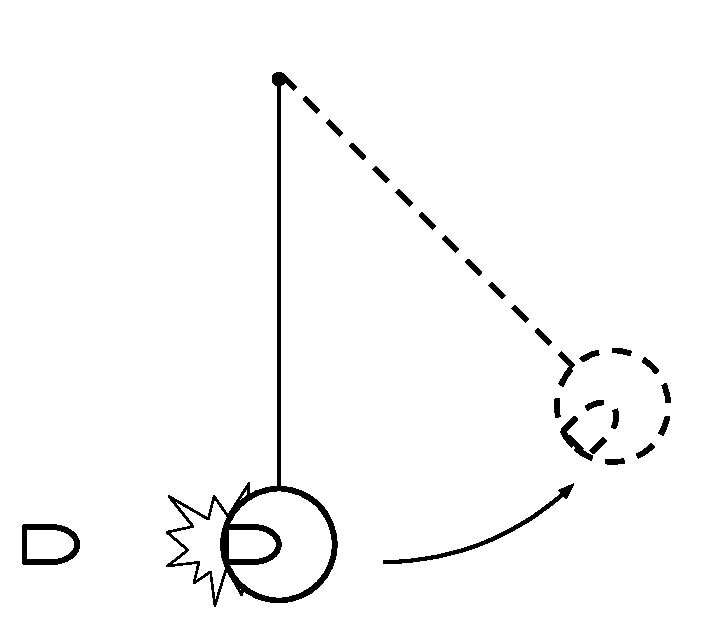
\includegraphics[width = \marginparwidth]{pballistico.pdf}
    \caption{Il pendolo balistico}
    \label{ballistico}
\end{marginfigure}
Un pendolo balistico è costituito da due elementi principali: Un
pendolo, costituito da un filo o asta al quale è agganciato un
bersaglio (spesso un sacco di sabbia o un blocco di legno),
e un proiettile. Generalmente, per funzionare bene, ci si aspetta
che la massa del proiettile sia relativamente ridotta rispetto a
quella del bersaglio. Per utilizzare il pendolo balistico, si
spara il proiettile verso il bersaglio fermo, in modo che la traiettoria
del proiettile sia perpendicolare al filo del pendolo. Quando il
proiettile colpisce il bersaglio, esso si conficca al suo interno
e il pendolo comincia ad oscillare per via dell'urto.

Il pendolo balistico è un metodo ingegnoso per misurare in
particolare la velocità del proiettile. Ciò che è sufficiente
conoscere sono le
masse del proiettile ($m$) e del bersaglio ($M$), l'altezza massima di
oscillazione del pendolo ($h$), a partire dalla posizione di equilibrio,
e l'accelerazione di gravità del pianeta
sul quale ci si trova (nel caso della Terra, $g$). Si consideri
l'istante immediatamente precedente all'urto proiettile-bersaglio:
in questo caso, la quantità di moto dell'intero sistema è data dalla
somma della quantità di moto del proiettile e quella del bersaglio
appeso al pendolo, ma sappiamo che quest'ultimo è fermo.

\[ \vecsymb{p}_i = m\vecsymb{v} + M\vec{0} = m\vecsymb{v} \]

\noindent Il proiettile si conficca nel bersaglio, rimanendovi incastrato.
Si tratta dunque di un urto idealmente anelastico. Stavolta il
pendolo comincerà a muoversi con una certa velocità $\vecsymb{V}$
ma la sua massa include quella del proiettile.

\[ \vecsymb{p}_f = (m + M)\vecsymb{V} \]

\noindent La quantità di moto del sistema si conserva e dunque
$\vecsymb{p}_i = \vecsymb{p}_f$, ma supponendo di voler ottenere $\vecsymb{v}$,
serve un'ulteriore
via per trovare l'incognita $\vecsymb{V}$. Per fare questo, ricorriamo alla
meccanica. Immediatamente dopo l'urto, il pendolo comincia
ad elevarsi ad una certa altezza $h$, che possiamo
facilmente misurare, dove il pendolo si fermerà per poi oscillare
ciclicamente. Supponiamo che l'energia cinetica del pendolo sia
massima nel punto di equilibrio e che invece la sua energia potenziale
sia nulla. All'altezza $h$, invece, l'energia cinetica è nulla, perché
il pendolo si ferma per invertire l'oscillazione, mentre l'energia
potenziale è massima. Dal momento che sul sistema solo le forze
conservative compiono lavoro (la forza peso), possiamo applicare il
principio di conservazione dell'energia meccanica.

\[ \Delta E = E_{K_f} + \mathcal{U}_f - (E_{k_i} + \mathcal{U}_i) = (m + M)gh - \frac12(m + M)\vecsymb{V}^2 = 0 \]

\noindent Da cui otteniamo il modulo di $\vecsymb{V}$.

\[ V = \sqrt{2gh} \]

\noindent Passando ai moduli, consapevoli del fatto che i vettori
di $\vecsymb{V}$ e $\vecsymb{v}$ hanno direzione perpendicolare al
filo del pendolo, ricaviamo facilmente il risultato
dall'equazione sulla conservazione della quantità di moto:

\[ v = \frac{m + M}{m}\sqrt{2gh} \]

\noindent Ovviamente questa equazione può essere invertita a piacere
a seconda del dato che si intende individuare, non necessariamente
la velocità del proiettile.


\subsection{Pendolo di Newton}

\subsection{Carrelli}